\documentclass[12pt,a4paper]{article}
\newcommand{\reportTitle}{Laboratory work 4:}
\newcommand{\reportSubject}{Study and Empirical Analysis of\\[0.3cm]Dijkstra and Floyd--Warshall Shortest Path Algorithms}
\usepackage{iftex}
\ifPDFTeX
    \usepackage[T1]{fontenc}
    \usepackage[utf8]{inputenc}
    \usepackage{mathptmx}
    \usepackage{courier}
\else
    \usepackage{fontspec}
    \setmainfont{Times New Roman}
    \setmonofont{Courier New}
\fi

\usepackage{amsmath}
\usepackage{graphicx}
\usepackage{float}
\usepackage[english]{babel}
\usepackage{indentfirst}
\usepackage{geometry}
\geometry{
    a4paper,
    left=20mm,
    right=10mm,
    top=20mm,
    bottom=20mm
}

\usepackage{setspace}
\setstretch{1.5}
\setlength{\parindent}{1.25cm}
\setlength{\parskip}{0pt}

\usepackage{titlesec}
\titleformat{\section}
  {\normalfont\bfseries\centering\fontsize{13}{15}\selectfont\MakeUppercase}{\thesection}{0.8em}{}
\titleformat{\subsection}
  {\normalfont\bfseries\fontsize{12}{14}\selectfont}{\thesubsection}{0.8em}{}
\titleformat{\subsubsection}
  {\normalfont\bfseries\fontsize{12}{14}\selectfont}{\thesubsubsection}{0.8em}{}

\titlespacing*{\section}{0pt}{0pt}{0.8\baselineskip}
\titlespacing*{\subsection}{0pt}{0.6\baselineskip}{0.3\baselineskip}
\titlespacing*{\subsubsection}{0pt}{0.4\baselineskip}{0.2\baselineskip}

\setcounter{secnumdepth}{3}

\usepackage{booktabs}
\usepackage{array}
\usepackage{longtable}
\usepackage{chngcntr}
\usepackage{caption}
\usepackage{subcaption}
\usepackage{enumitem}
\usepackage{needspace}
\usepackage{xcolor}
\usepackage{listings}
\usepackage{tocloft}

\setlist[itemize]{label=--,leftmargin=1.25cm,itemsep=0pt,topsep=0pt}
\setlist[enumerate]{leftmargin=1.25cm,itemsep=0pt,topsep=0pt}

\renewcommand{\cftsecleader}{\cftdotfill{1}}
\renewcommand{\cftsubsecleader}{\cftdotfill{1}}
\renewcommand{\cftsubsubsecleader}{\cftdotfill{1}}
\setlength{\cftbeforesecskip}{0pt}
\setlength{\cftbeforesubsecskip}{0pt}
\setlength{\cftbeforesubsubsecskip}{0pt}
\setlength{\cftsecindent}{0pt}
\setlength{\cftsubsecindent}{0.5cm}
\setlength{\cftsubsubsecindent}{1cm}
\setlength{\cftsecnumwidth}{1.0cm}
\setlength{\cftsubsecnumwidth}{1.0cm}
\setlength{\cftsubsubsecnumwidth}{1.2cm}
\renewcommand{\cftsecfont}{\bfseries}
\renewcommand{\cftsubsecfont}{\normalfont}
\renewcommand{\cftsecpagefont}{\bfseries}
\renewcommand{\cftsubsecpagefont}{\normalfont}
\renewcommand{\cfttoctitlefont}{\hfill\normalfont\Large\bfseries}
\renewcommand{\cftaftertoctitle}{\hfill}
\setcounter{tocdepth}{2}

\usepackage{hyperref}
\usepackage{bookmark}
\hypersetup{
    hidelinks,
    linktoc=all
}
\addto\captionsenglish{\renewcommand{\contentsname}{TABLE OF CONTENTS}}
\renewcommand{\contentsname}{TABLE OF CONTENTS}

\counterwithin{figure}{section}
\counterwithin{table}{section}
\counterwithin{equation}{section}

\newcommand{\reportcodestyle}{\linespread{1}\ttfamily\fontsize{10}{10}\selectfont}

\lstset{
    basicstyle=\reportcodestyle,
    frame=none,
    breaklines=true,
    columns=fullflexible,
    keepspaces=true,
    showstringspaces=false,
    aboveskip=0.2\baselineskip,
    belowskip=0.2\baselineskip
}

\captionsetup[figure]{
    font=bf,
    labelfont=bf,
    textfont=bf,
    labelsep=endash,
    justification=centering,
    singlelinecheck=false
}
\captionsetup[table]{
    font=normalfont,
    labelfont=normalfont,
    textfont=normalfont,
    labelsep=endash,
    justification=raggedleft,
    singlelinecheck=false,
    position=above
}

\newcommand{\studentName}{Ple\c{s}u Dinu}
\newcommand{\studentGroup}{FAF-241}
\newcommand{\teacherTitle}{asist. univ.}
\newcommand{\teacherName}{Fi\c{s}tic Cristofor}
\newcommand{\reportYear}{2026}
\newcommand{\reportCity}{Chi\c{s}in\u{a}u}

\newcommand{\makelabtitle}{
    \begin{titlepage}
        \centering

        \textbf{\large Ministerul Educa\c{t}iei \c{s}i Cercet\u{a}rii al Republicii Moldova}\\[0.3cm]
        \textbf{\large Universitatea Tehnic\u{a} a Moldovei}\\[0.3cm]
        \textbf{\large Facultatea Calculatoare, Informatic\u{a} \c{s}i Microelectronic\u{a}}\\[3cm]

        \vfill

        {\LARGE \reportTitle}\\[0.5cm]
        {\LARGE \reportSubject}\\[3cm]

        \vfill

        \begin{flushleft}
            \hspace{1cm}
            \begin{minipage}{0.8\textwidth}
                {\large Elaborated:}\\
                {\large st.\ gr.\ \studentGroup \hfill \studentName}\\[0.8cm]
                {\large Verified:}\\
                {\large \teacherTitle \hfill \teacherName}\\
            \end{minipage}
        \end{flushleft}

        \vfill

        {\large \reportCity\ - \reportYear}
    \end{titlepage}
}

\newcommand{\startreport}{
    \begin{document}
    \makelabtitle
    \newpage
    \pagenumbering{arabic}
    \setcounter{page}{2}
    \thispagestyle{empty}
    \tableofcontents
    \thispagestyle{empty}
    \newpage
}

\newcommand{\reportprelimsection}[1]{
    \newpage
    \section*{#1}
    \thispagestyle{empty}
    \phantomsection
    \addcontentsline{toc}{section}{#1}
}

\newcommand{\reportintroduction}{
    \newpage
    \section*{INTRODUCTION}
    \phantomsection
    \addcontentsline{toc}{section}{INTRODUCTION}
}

\newcommand{\reportmainsection}[1]{
    \newpage
    \section{#1}
}

\newcommand{\tocsubsection}[1]{
    \Needspace{12\baselineskip}
    \subsection{#1}
}

\newcommand{\reportlabel}[1]{
    \Needspace{6\baselineskip}
    \par\noindent\textbf{#1}\par
}

\newcommand{\reportfrontsubsection}[1]{
    \subsection*{#1}
    \phantomsection
    \addcontentsline{toc}{subsection}{#1}
}

\newcommand{\reportunnumberedsection}[1]{
    \newpage
    \section*{#1}
    \phantomsection
    \addcontentsline{toc}{section}{#1}
}

\newcommand{\reportreferences}[1]{
    \newpage
    \section*{REFERENCES}
    \phantomsection
    \addcontentsline{toc}{section}{REFERENCES}
    \begin{thebibliography}{99}
    #1
    \end{thebibliography}
}


\startreport


\reportintroduction
Finding the shortest path between vertices in a weighted graph is one of the most practically important problems in computer science. Applications span network routing protocols, where routers continuously compute minimum-cost paths through dynamic topologies; geographic navigation systems that determine optimal driving routes across road networks with millions of nodes; resource allocation in operations research; and reachability analysis in compiler data-flow problems. In each of these domains, the ability to compute minimum-cost connections efficiently can mean the difference between a system that scales to real-world input sizes and one that does not.

The shortest-path problem comes in two principal variants. The single-source shortest-path problem asks for the minimum-cost path from one designated source vertex to all other vertices reachable from it. The all-pairs shortest-path problem asks for the minimum-cost path between every ordered pair of vertices in the graph. These two variants require fundamentally different algorithmic approaches and exhibit very different scaling behaviour as the graph grows.

Dijkstra's algorithm solves the single-source problem on graphs with non-negative edge weights by maintaining a set of finalized vertices and repeatedly selecting the closest unfinalized vertex. The priority of each remaining vertex is relaxed whenever a shorter path is discovered through a newly finalized vertex. The correctness of this greedy relaxation strategy rests on the non-negativity of weights: if all edge weights are non-negative, a path cannot be shortened by extending it, so the first time a vertex is finalized its distance is already optimal. Two implementation strategies are studied: the classic linear-scan variant and an optimized heap-based variant.

The Floyd--Warshall algorithm solves the all-pairs problem using a dynamic-programming recurrence. It considers all vertices as potential intermediate nodes one by one and updates the distance matrix whenever routing through the current intermediate vertex improves a previously known path. Because it must consider all ordered pairs for each intermediate vertex, its time complexity is cubic in the number of vertices, making it practical only for substantially smaller inputs than Dijkstra.

Both algorithms were tested on weighted directed graphs spanning several size and density categories. Dijkstra was benchmarked on graphs with up to 1500 nodes, while Floyd--Warshall was limited to smaller inputs where its cubic cost is still manageable. The main goal was to check whether the observed scaling matches theoretical predictions and to measure the practical gain of each optimized implementation over the naive one.

\reportmainsection{ALGORITHM ANALYSIS}

\tocsubsection{Objective}
Study and analyze Dijkstra and Floyd--Warshall on weighted directed graphs with different sizes and densities.

\tocsubsection{Tasks}
\begin{enumerate}[leftmargin=1.25cm]
    \item study the dynamic-programming method of designing algorithms;
    \item implement Dijkstra and Floyd--Warshall in a programming language;
    \item perform empirical analysis for sparse and dense graphs;
    \item increase the number of nodes and analyze the influence on the algorithms;
    \item make a graphical presentation of the obtained data;
    \item formulate conclusions.
\end{enumerate}

\tocsubsection{Theoretical Notes}
Empirical analysis complements theoretical complexity analysis by providing concrete measurements of algorithm behaviour on real hardware. Theoretical analysis establishes asymptotic bounds, but constants, cache behaviour, memory allocation patterns, and language interpreter overhead can cause the observed running times to deviate significantly from what a simple complexity expression predicts. In this laboratory, the purpose of empirical analysis is therefore both to confirm that the theoretical complexity class is visible in the data and to quantify the practical advantage of optimized implementations over their naive counterparts \cite{gfg-dp,tp-dp}.

Dynamic programming is an algorithm design paradigm that solves a problem by decomposing it into overlapping subproblems, solving each subproblem exactly once, and storing the results so that they can be reused without recomputation. The key requirements for dynamic programming applicability are optimal substructure, meaning that an optimal solution to the problem contains optimal solutions to its subproblems, and overlapping subproblems, meaning that the same subproblem recurs many times during the computation. Both Dijkstra and Floyd--Warshall exploit optimal substructure of shortest paths: a shortest path from vertex \(i\) to vertex \(j\) through intermediate vertex \(k\) consists of a shortest path from \(i\) to \(k\) concatenated with a shortest path from \(k\) to \(j\).

Dijkstra's algorithm maintains a distance array \(d[v]\) for each vertex \(v\), initialized to \(\infty\) for all vertices except the source which is set to \(0\). At each step the unfinalized vertex with the smallest current distance is selected and its outgoing edges are relaxed: for each edge \((u, v, w)\), if \(d[u] + w < d[v]\) then \(d[v]\) is updated to \(d[u] + w\). The classic implementation selects the minimum-distance vertex by a linear scan of all unfinalized vertices, costing \(O(V)\) per selection and \(O(V^2)\) in total over all \(V\) iterations. The optimized implementation stores unfinalized vertices in a binary min-heap, reducing the selection cost to \(O(\log V)\) and each relaxation to \(O(\log V)\), giving an overall complexity of \(O((V + E)\log V)\). On sparse graphs where \(E = O(V)\) the heap variant is decisively faster, while on dense graphs where \(E = O(V^2)\) the linear-scan variant can compete because the heap incurs \(O(E \log V) = O(V^2 \log V)\) relaxation updates.

Floyd--Warshall initializes a distance matrix \(dist[i][j]\) with the direct edge weight between vertices \(i\) and \(j\), or \(\infty\) if no edge exists, and \(0\) on the diagonal. The algorithm then iterates over all vertices \(k\) from \(1\) to \(n\) and applies the recurrence \(dist[i][j] = \min(dist[i][j],\, dist[i][k] + dist[k][j])\) for all pairs \((i, j)\). After all \(n\) iterations, \(dist[i][j]\) holds the shortest-path distance between every ordered pair. The time complexity is \(\Theta(V^3)\) and the space complexity is \(\Theta(V^2)\). The algorithm is correct on graphs without negative-weight cycles; the presence of a negative-weight cycle causes some diagonal entries to become negative after the iterations complete, which can be used as a detection criterion. The optimized variant skips the inner pair \((i, j)\) whenever \(dist[i][k]\) or \(dist[k][j]\) is \(\infty\), reducing unnecessary work on sparse distance matrices \cite{cn}.

The practical data structure choices have a decisive effect on performance. For Dijkstra, the transition from a linear-scan minimum selection to a binary heap changes the bottleneck from vertex selection to edge relaxation, and the observed speedup is proportional to the ratio \(V / \log V\). For Floyd--Warshall, the bottleneck is the triple nested loop over all triples \((k, i, j)\), which runs unconditionally in the classic version. The optimized variant breaks out of the inner loops when intermediate distances are infinite, which provides substantial savings on sparse graphs where most entries remain at \(\infty\) throughout the computation.

\tocsubsection{Comparison Metric}
Four values were recorded for each run:
\begin{itemize}[leftmargin=1.25cm]
    \item execution time in milliseconds;
    \item peak memory usage in kilobytes;
    \item number of reachable distances;
    \item number of edges and graph density.
\end{itemize}

\tocsubsection{Input Format}
The benchmark used weighted directed graphs with positive integer weights from 1 to 20. Three graph categories were generated:
\begin{itemize}[leftmargin=1.25cm]
    \item sparse graphs;
    \item medium-density graphs;
    \item dense graphs.
\end{itemize}

For Dijkstra, the tested sizes were 100, 250, 500, 1000, and 1500 nodes. For Floyd--Warshall, the tested sizes were 25, 50, 75, 100, and 125 nodes.

\reportmainsection{IMPLEMENTATION}

\tocsubsection{Dijkstra}
Two Dijkstra variants were implemented: a classic one based on linear minimum selection, and an optimized one using a priority queue. Both were tested on the same generated weighted directed graphs \cite{repo}.

\subsubsection{Algorithm Description}

The method follows the idea shown in the next pseudocode.

\begin{lstlisting}
Dijkstra(graph, source):
    set distance[source] = 0
    set all other distances to infinity
    while there are unprocessed vertices:
        choose the vertex with minimum distance
        relax all outgoing edges from that vertex
    return distance array
\end{lstlisting}

\subsubsection{Implementation}

The key difference between the two is how the next vertex to process is chosen. The classic approach scans all unvisited vertices on each step; the optimized approach uses a heap instead, trading memory for a significant reduction in per-step cost.

\begin{lstlisting}
# Classic -- O(V^2) linear minimum selection
def dijkstra_classic(graph, source=0):
    n = graph.num_vertices
    distances = [INF] * n
    visited = [False] * n
    distances[source] = 0
    for _ in range(n):
        current = -1
        for v in range(n):
            if not visited[v] and (current == -1
                    or distances[v] < distances[current]):
                current = v
        if current == -1:
            break
        visited[current] = True
        for neighbor, weight in graph.adj[current]:
            if distances[current] + weight < distances[neighbor]:
                distances[neighbor] = distances[current] + weight
    return distances

# Optimized -- O((V+E) log V) heap-based priority queue
def dijkstra_optimized(graph, source=0):
    distances = [INF] * graph.num_vertices
    distances[source] = 0
    heap = [(0, source)]
    while heap:
        dist, vertex = heapq.heappop(heap)
        if dist != distances[vertex]:
            continue
        for neighbor, weight in graph.adj[vertex]:
            if dist + weight < distances[neighbor]:
                distances[neighbor] = dist + weight
                heapq.heappush(heap, (distances[neighbor], neighbor))
    return distances
\end{lstlisting}

\subsubsection{Results}

The representative results at the largest tested size (1500 nodes) are shown in Table~\ref{tab:lab4-dijkstra}.

\begin{table}[H]
    \caption{Dijkstra benchmark at 1500 nodes}
    \label{tab:lab4-dijkstra}
    \centering
    {\fontsize{11}{11}\selectfont\renewcommand{\arraystretch}{1}\begin{tabular}{lllll}
\toprule
Graph type & Algorithm & Time (ms) & Memory (KB) & Edges \\
\midrule
dense & Dijkstra\_Classic & 4562.149 & 23.66 & 1461720.0 \\
dense & Dijkstra\_Optimized & 226.503 & 209.75 & 1461720.0 \\
sparse & Dijkstra\_Classic & 3325.892 & 23.66 & 337166.0 \\
sparse & Dijkstra\_Optimized & 53.918 & 175.16 & 337166.0 \\
\bottomrule
\end{tabular}
}
\end{table}

As Table~\ref{tab:lab4-dijkstra} shows, the difference is substantial: on the 1500-node dense graph (1\,461\,720 edges) the classic variant took \(4562.1\) ms while the optimized one finished in \(226.5\) ms. Figure~\ref{fig:lab4-dijkstra} shows how this gap develops with graph size.

\begin{figure}[H]
    \centering
    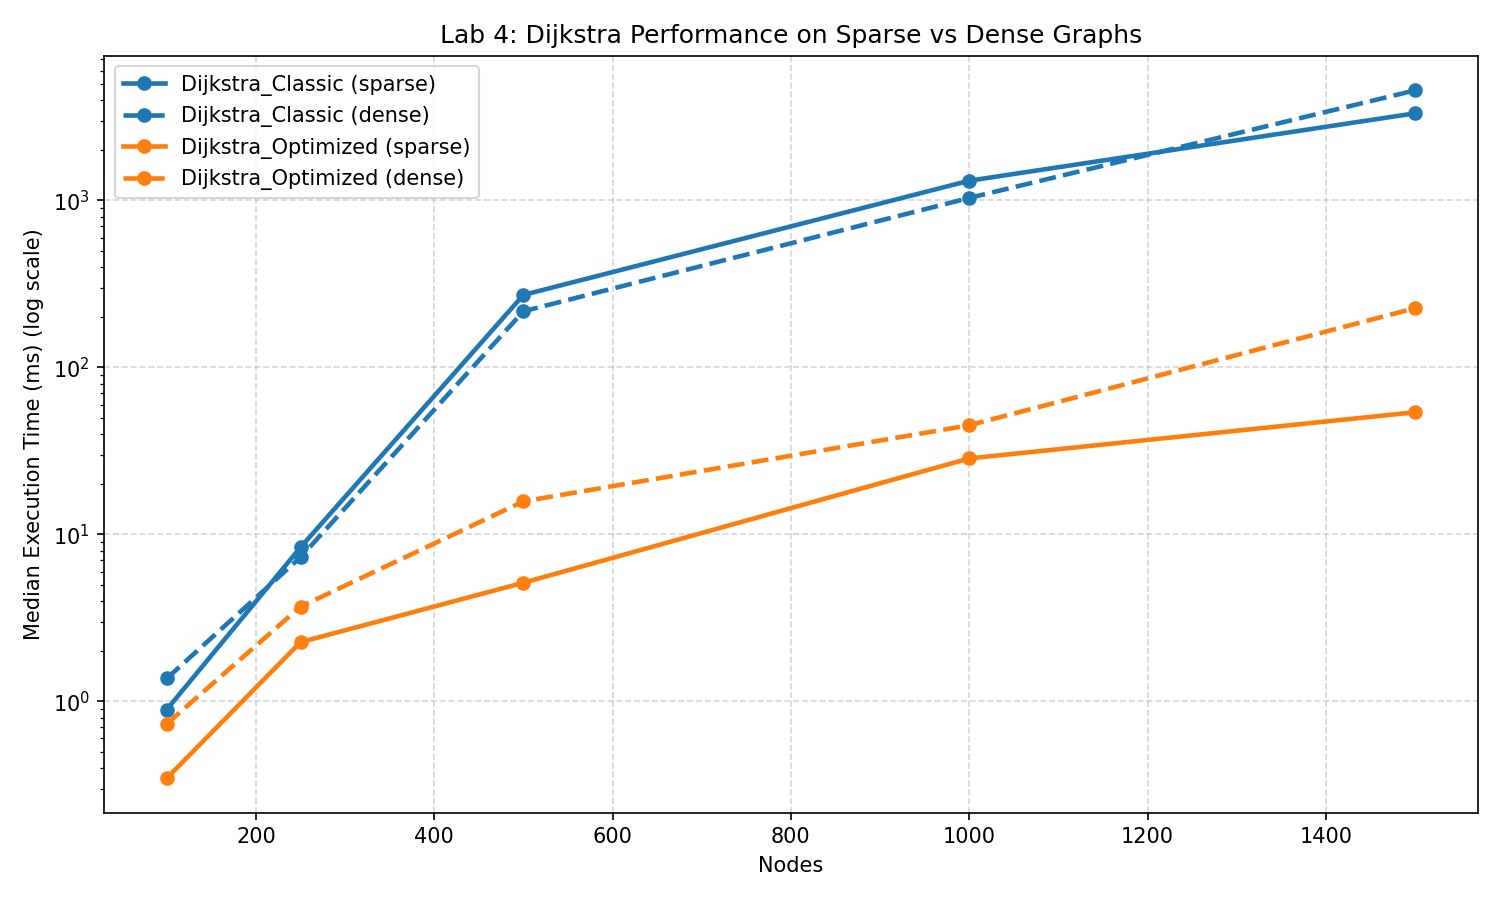
\includegraphics[width=0.88\textwidth]{../../Lab4/plots/dijkstra_sparse_dense_performance.png}
    \caption{Dijkstra performance on sparse and dense graphs}
    \label{fig:lab4-dijkstra}
\end{figure}

A logarithmic scale is used because the performance gap becomes very large at higher node counts.

\subsubsection{Conclusion}

Dijkstra is well suited for large weighted graphs when shortest paths from a single source are required. On the 1500-node dense graph with 1\,461\,720 edges, the classic implementation required \(4562.1\) ms while the optimized implementation required only \(226.5\) ms, a speedup factor of approximately \(20\times\). Across the full benchmark suite the optimized implementation is on average \(28.5\times\) faster than the classic, confirming that the \(O(\log V)\) heap operation dominates over the \(O(V)\) linear scan as the graph grows.

\tocsubsection{Floyd--Warshall}
Two Floyd--Warshall variants were also implemented: a classic triple-loop version and an optimized one that skips unreachable intermediate vertices. Both solve the all-pairs problem and were tested on the same graph categories.

\subsubsection{Algorithm Description}

The Floyd--Warshall method follows the recurrence shown in the next pseudocode.

\begin{lstlisting}
FloydWarshall(matrix):
    dist = matrix copy
    for k from 1 to n:
        for i from 1 to n:
            for j from 1 to n:
                dist[i][j] = min(dist[i][j], dist[i][k] + dist[k][j])
    return dist
\end{lstlisting}

\subsubsection{Implementation}

In principle, skipping unreachable intermediate nodes should save inner-loop iterations on sparse graphs. In practice the Python interpreter's branch overhead partly cancels this benefit, so the measured gains are smaller than the complexity argument alone would suggest.

\begin{lstlisting}
# Classic -- O(V^3) triple nested loop
def floyd_warshall_classic(graph):
    dist = graph.to_matrix()
    n = graph.num_vertices
    for k in range(n):
        for i in range(n):
            for j in range(n):
                if dist[i][k] + dist[k][j] < dist[i][j]:
                    dist[i][j] = dist[i][k] + dist[k][j]
    return dist

# Optimized -- skips unreachable intermediate vertices
def floyd_warshall_optimized(graph):
    dist = graph.to_matrix()
    n = graph.num_vertices
    for k in range(n):
        for i in range(n):
            if dist[i][k] == INF:
                continue
            for j in range(n):
                if dist[k][j] != INF:
                    if dist[i][k] + dist[k][j] < dist[i][j]:
                        dist[i][j] = dist[i][k] + dist[k][j]
    return dist
\end{lstlisting}

\subsubsection{Results}

The results at the largest Floyd--Warshall input (125 nodes) are shown in Table~\ref{tab:lab4-floyd}.

\begin{table}[H]
    \caption{Floyd--Warshall benchmark at 125 nodes}
    \label{tab:lab4-floyd}
    \centering
    {\fontsize{11}{11}\selectfont\renewcommand{\arraystretch}{1}\begin{tabular}{lllll}
\toprule
Graph type & Algorithm & Time (ms) & Memory (KB) & Edges \\
\midrule
dense & FloydWarshall\_Classic & 440.023 & 125.85 & 10169.0 \\
dense & FloydWarshall\_Optimized & 728.650 & 125.80 & 10169.0 \\
sparse & FloydWarshall\_Classic & 650.790 & 125.85 & 2337.0 \\
sparse & FloydWarshall\_Optimized & 625.741 & 125.80 & 2337.0 \\
\bottomrule
\end{tabular}
}
\end{table}

As Table~\ref{tab:lab4-floyd} shows, the gap between the two Floyd--Warshall variants is much smaller than for Dijkstra, and on dense graphs the classic variant actually came out ahead. Figure~\ref{fig:lab4-floyd} illustrates the growth pattern.

\begin{figure}[H]
    \centering
    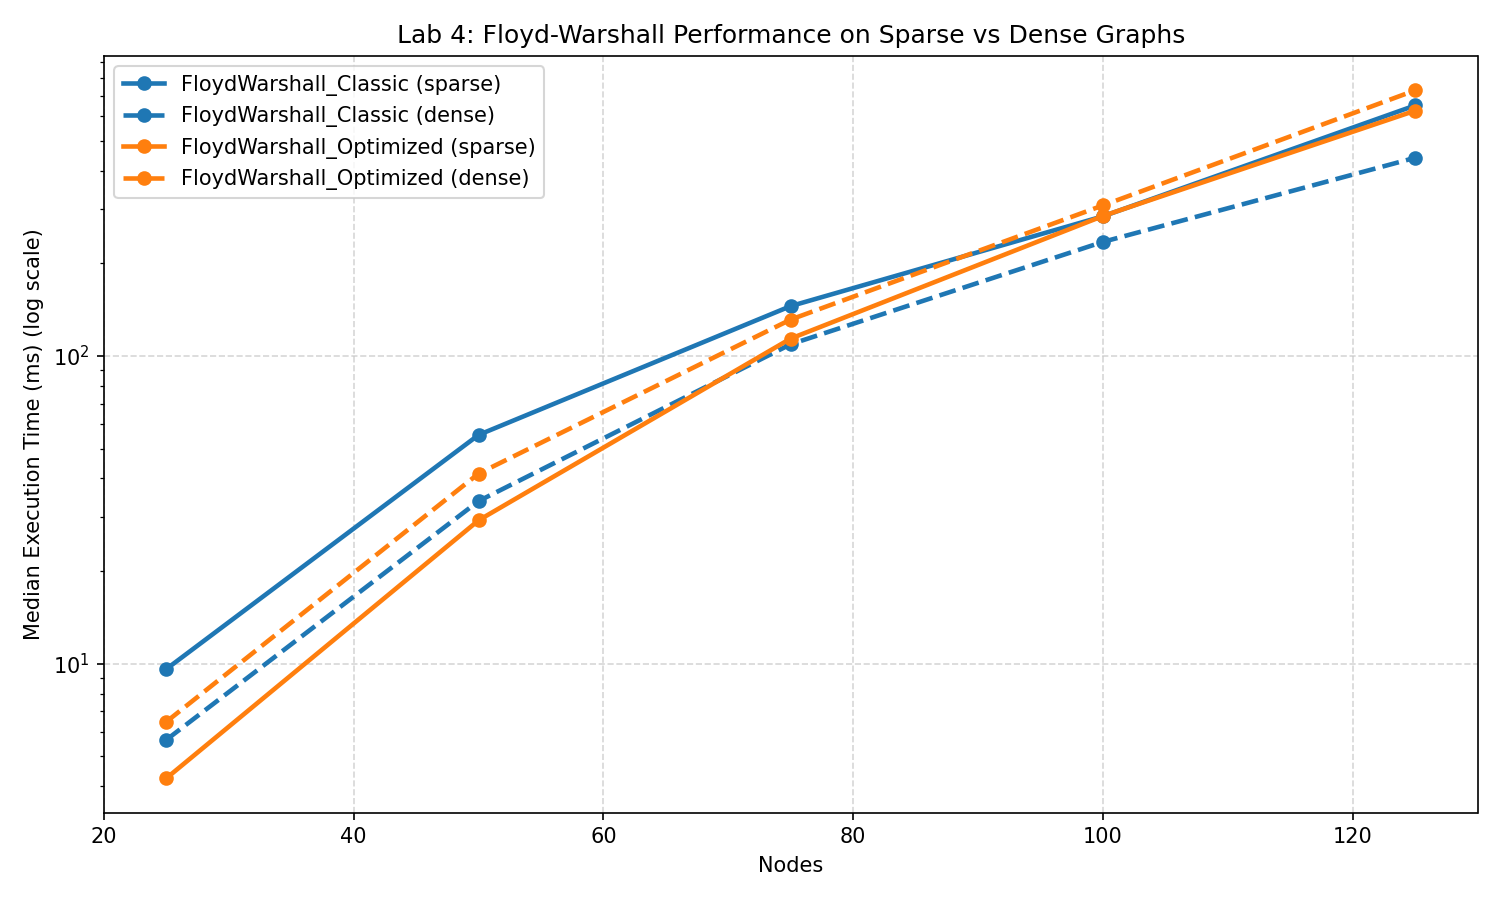
\includegraphics[width=0.88\textwidth]{../../Lab4/plots/floyd_warshall_sparse_dense_performance.png}
    \caption{Floyd--Warshall performance on sparse and dense graphs}
    \label{fig:lab4-floyd}
\end{figure}

Even at these small node counts the cubic growth is already noticeable --- running time roughly doubled with each step up in graph size.

\subsubsection{Conclusion}

Floyd--Warshall remains correct and useful for all-pairs shortest-path queries on small graphs, but its cubic growth is immediately visible in the data. At 125 nodes the classic variant required \(440.0\) ms on dense graphs. Unexpectedly, the optimized variant was slower than the classic on dense and medium inputs: at 125 dense nodes the optimized required \(728.6\) ms against the classic's \(440.0\) ms, because the additional conditional tests introduce branch-prediction penalties that outweigh the savings from skipping iterations when most distance-matrix entries are finite. Only on sparse graphs, where many entries remain at \(\infty\), did the optimized variant produce a net gain: \(625.7\) ms versus the classic's \(650.8\) ms at 125 sparse nodes.

\tocsubsection{Comparative Analysis}

Since Dijkstra and Floyd--Warshall solve different problem variants and ran on very different input sizes, comparing their raw running times would not be meaningful. It is more useful to look at each algorithm separately and consider how density and implementation choices affect its performance.

Figure~\ref{fig:lab4-dijkstra-all} shows both Dijkstra variants across all tested graph types. The heap variant consistently comes out ahead at every size and density, with the gap widening as the graph grows. Interestingly, sparse graphs show the largest relative advantage: with fewer edges to relax, the classic variant's linear scan wastes proportionally more time on empty visits.

\begin{figure}[H]
    \centering
    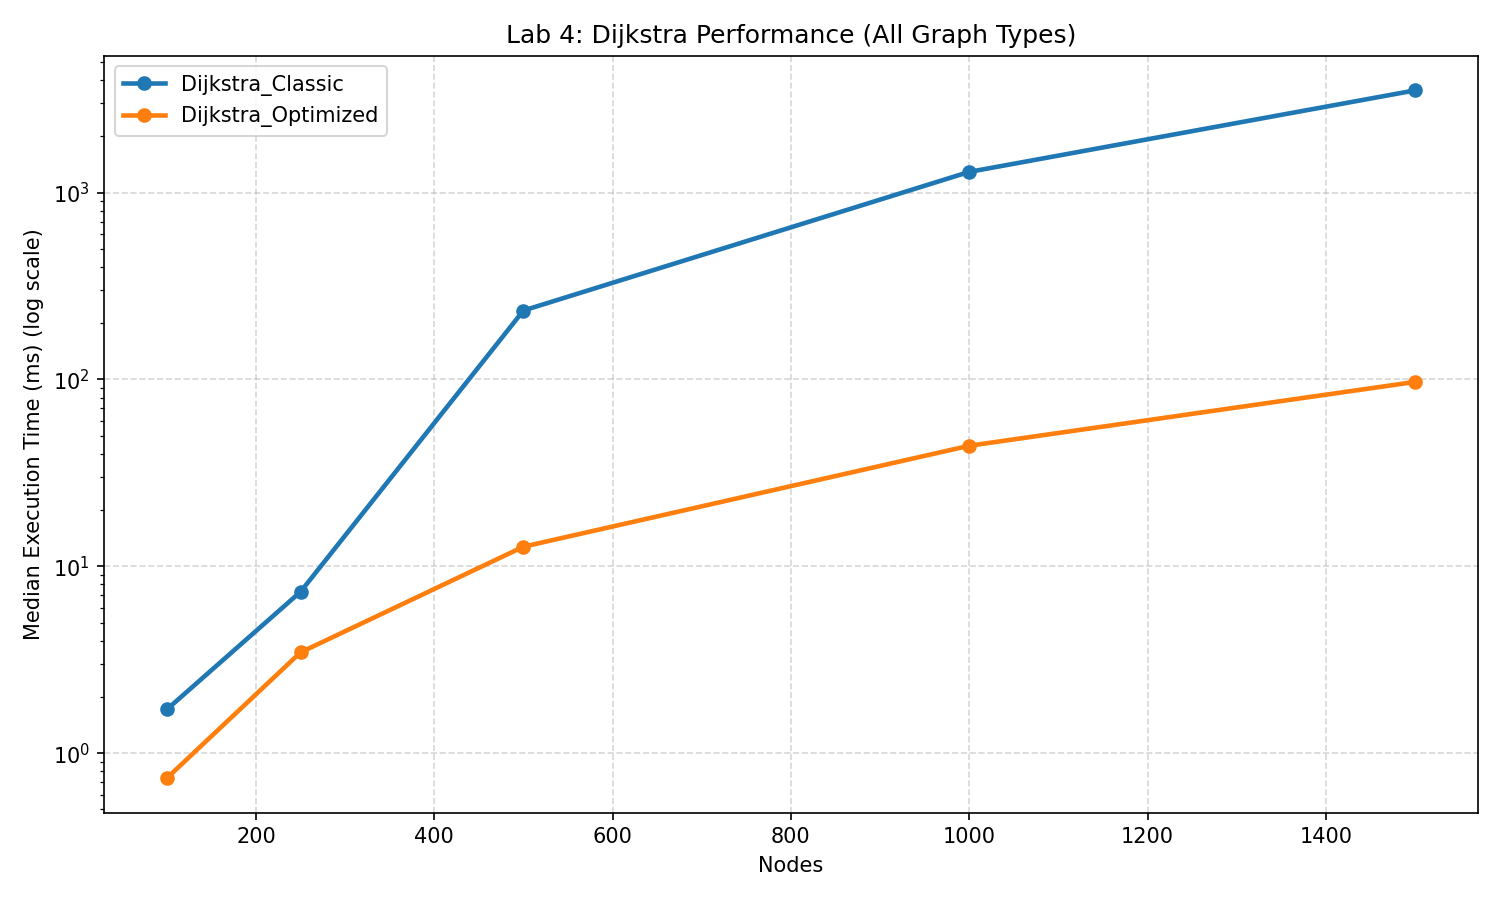
\includegraphics[width=0.88\textwidth]{../../Lab4/plots/dijkstra_performance.png}
    \caption{Dijkstra overall performance across all graph types}
    \label{fig:lab4-dijkstra-all}
\end{figure}

Figure~\ref{fig:lab4-fw-type} shows how density affects Floyd--Warshall. On sparse graphs the optimized variant benefits because many distance entries stay at \(\infty\) and the inner loop can be skipped early. As density rises, those entries fill in and the skipping condition fires less often, so the overhead of the extra checks eventually outweighs the savings.

\begin{figure}[H]
    \centering
    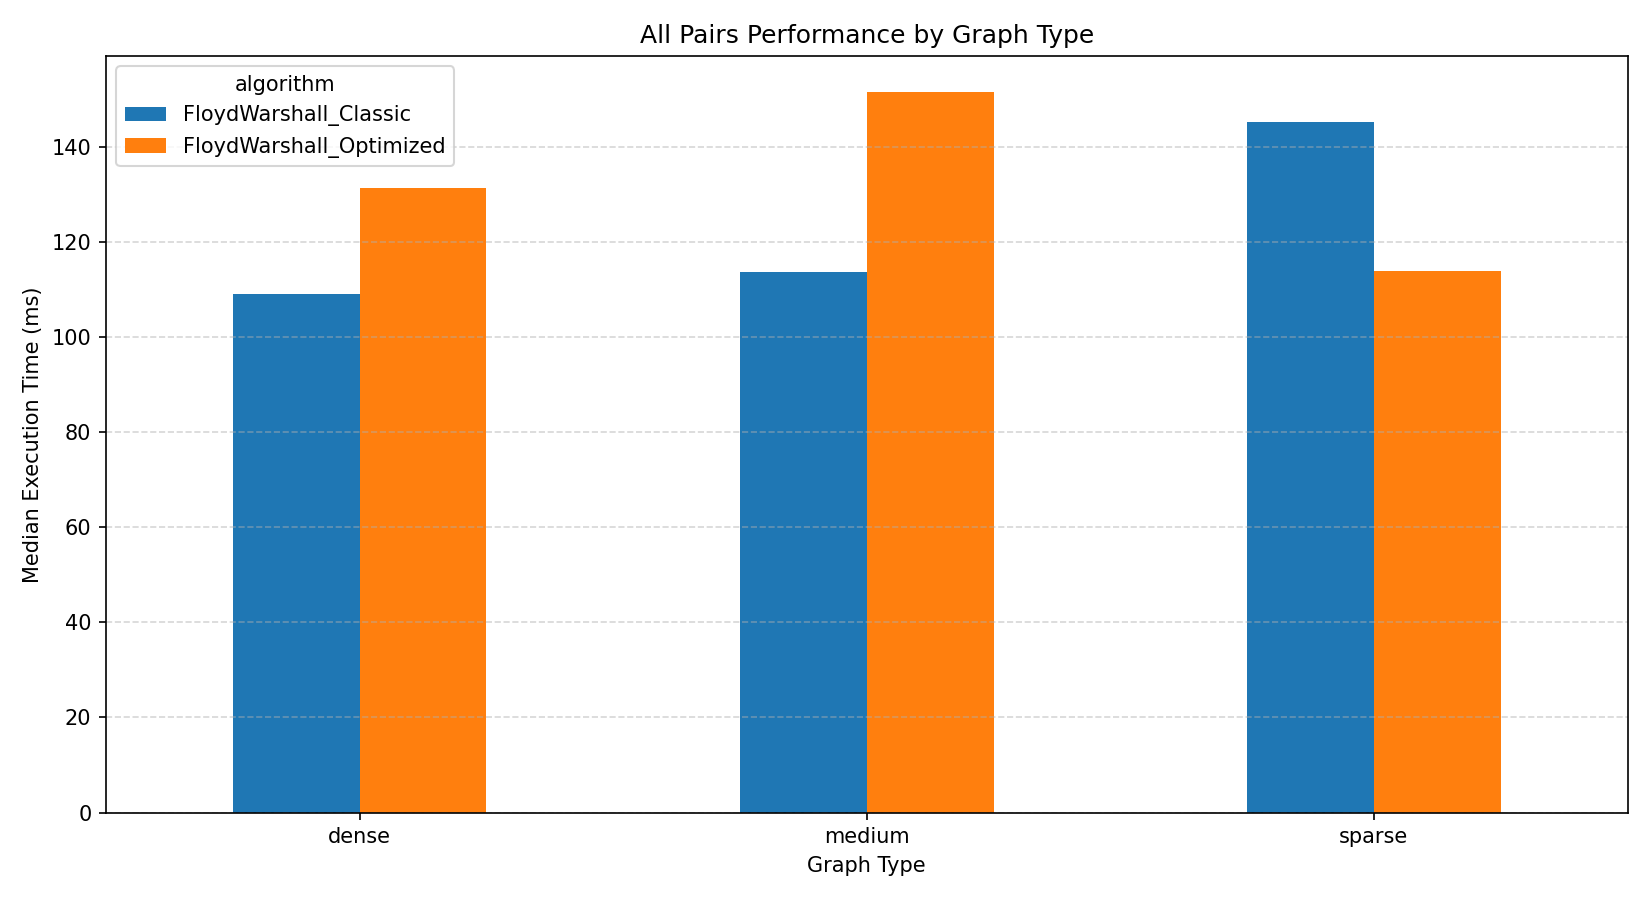
\includegraphics[width=0.88\textwidth]{../../Lab4/plots/floyd_warshall_by_graph_type.png}
    \caption{Floyd--Warshall performance by graph type}
    \label{fig:lab4-fw-type}
\end{figure}

Memory tells a different story. As Figure~\ref{fig:lab4-dijkstra-mem} shows, the heap-based Dijkstra is far more memory-hungry: on the 1500-node dense graph it consumed around \(210\) KB, while the classic variant needed only \(24\) KB. The priority queue accumulates pending vertices with their estimated distances, and this grows large on dense graphs.

\begin{figure}[H]
    \centering
    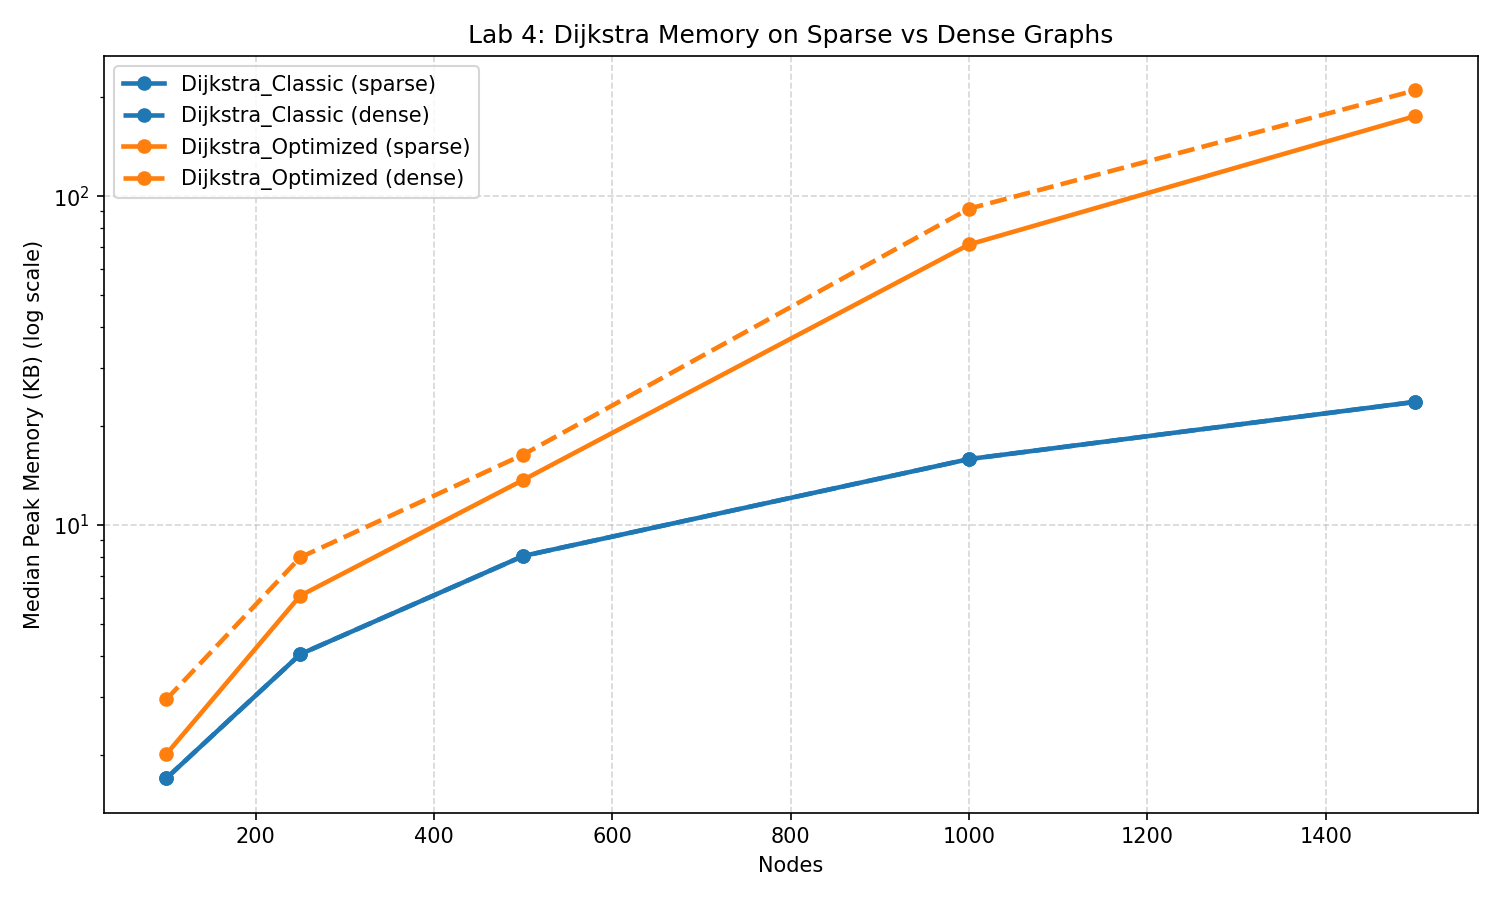
\includegraphics[width=0.88\textwidth]{../../Lab4/plots/dijkstra_sparse_dense_memory.png}
    \caption{Dijkstra memory usage on sparse and dense graphs}
    \label{fig:lab4-dijkstra-mem}
\end{figure}

Floyd--Warshall's memory depends entirely on the \(V \times V\) distance matrix, regardless of edge count. As Figure~\ref{fig:lab4-fw-mem} shows, both variants use nearly the same memory at each node count --- around \(126\) KB at 125 nodes for every density level. Density has no effect here because the matrix is always fully allocated.

\begin{figure}[H]
    \centering
    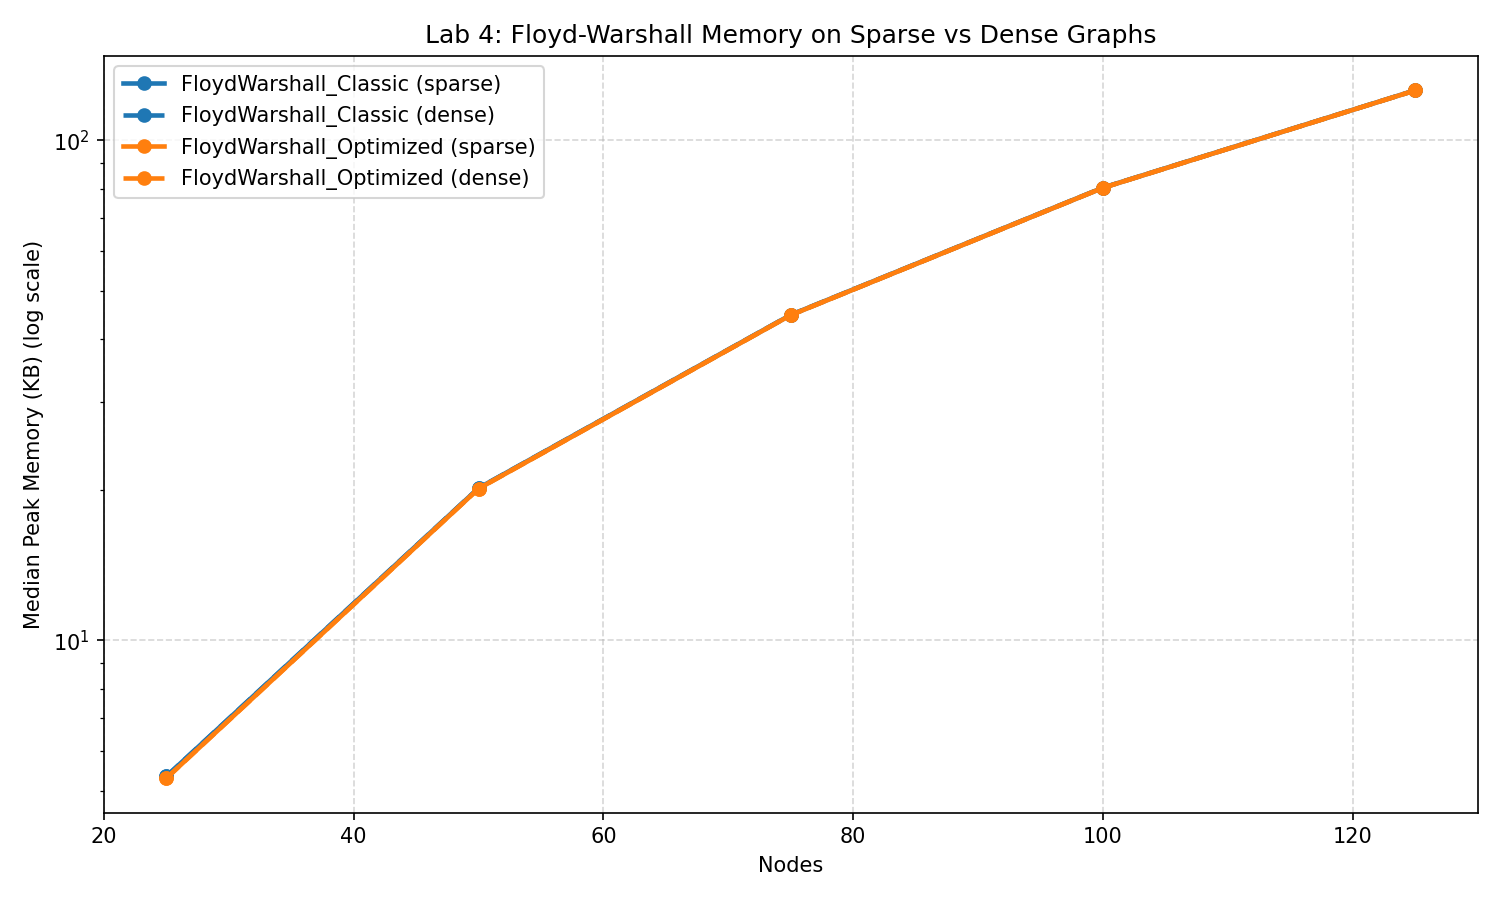
\includegraphics[width=0.88\textwidth]{../../Lab4/plots/floyd_warshall_sparse_dense_memory.png}
    \caption{Floyd--Warshall memory usage on sparse and dense graphs}
    \label{fig:lab4-fw-mem}
\end{figure}

\reportunnumberedsection{CONCLUSION}
Graph density and size had a clear effect on both algorithms throughout the benchmark. Dijkstra scales well for single-source queries: the heap-based variant averaged a \(28.5\times\) speedup over the classic across all tested inputs. Floyd--Warshall, limited by its \(O(V^3)\) cost, is only practical on small graphs and showed marginal or even negative gains from the Python-level optimization.

The sparse-versus-dense comparison was particularly informative. For Dijkstra, density increases the number of edge-relaxation operations, but the logarithmic cost of heap operations ensures that the optimized implementation scales well regardless of density. For Floyd--Warshall, sparse graphs allow the optimized variant to skip a meaningful fraction of inner-loop iterations, while dense graphs negate this benefit entirely. The practical implication is that the optimized Floyd--Warshall variant should be used only when graph density is known to be low.

The memory difference is worth noting. The heap-based Dijkstra uses around \(210\) KB at 1500 dense nodes versus \(24\) KB for the classic --- a real cost for the speed gain. Floyd--Warshall always uses \(\Theta(V^2)\) memory regardless of which variant is run. The practical guideline is straightforward: for large single-source problems use the optimized Dijkstra; for small all-pairs problems the classic Floyd--Warshall is the more predictable choice.

\reportreferences{
\bibitem{gfg-dp}
GeeksforGeeks. \textit{Dynamic Programming} [online]. [cited 07.05.2026]. Available: \url{https://www.geeksforgeeks.org/dynamic-programming/}.

\bibitem{tp-dp}
TutorialsPoint. \textit{Dynamic Programming} [online]. [cited 07.05.2026]. Available: \url{https://www.tutorialspoint.com/data_structures_algorithms/dynamic_programming.htm}.

\bibitem{cn}
Coding Ninjas. \textit{Dijkstra's Algorithm vs Floyd--Warshall's Algorithm} [online]. [cited 07.05.2026]. Available: \url{https://www.codingninjas.com/codestudio/library/dijkstras-algorithm-vs-floydwarshalls-algorithm}.

\bibitem{repo}
Ple\c{s}u D. \textit{aa-course-repo, Lab 4 source folder} [online]. GitHub, 2026. [cited 07.05.2026]. Available: \url{https://github.com/Prince-of-Nothing/aa-course-repo/tree/main/Lab4}.
}

\end{document}
